\chapter{IO Virtualization}
\label{chap:virt}

\begin{figure*}[!ht]
  \centering
    \subfloat[Emulation ]{
      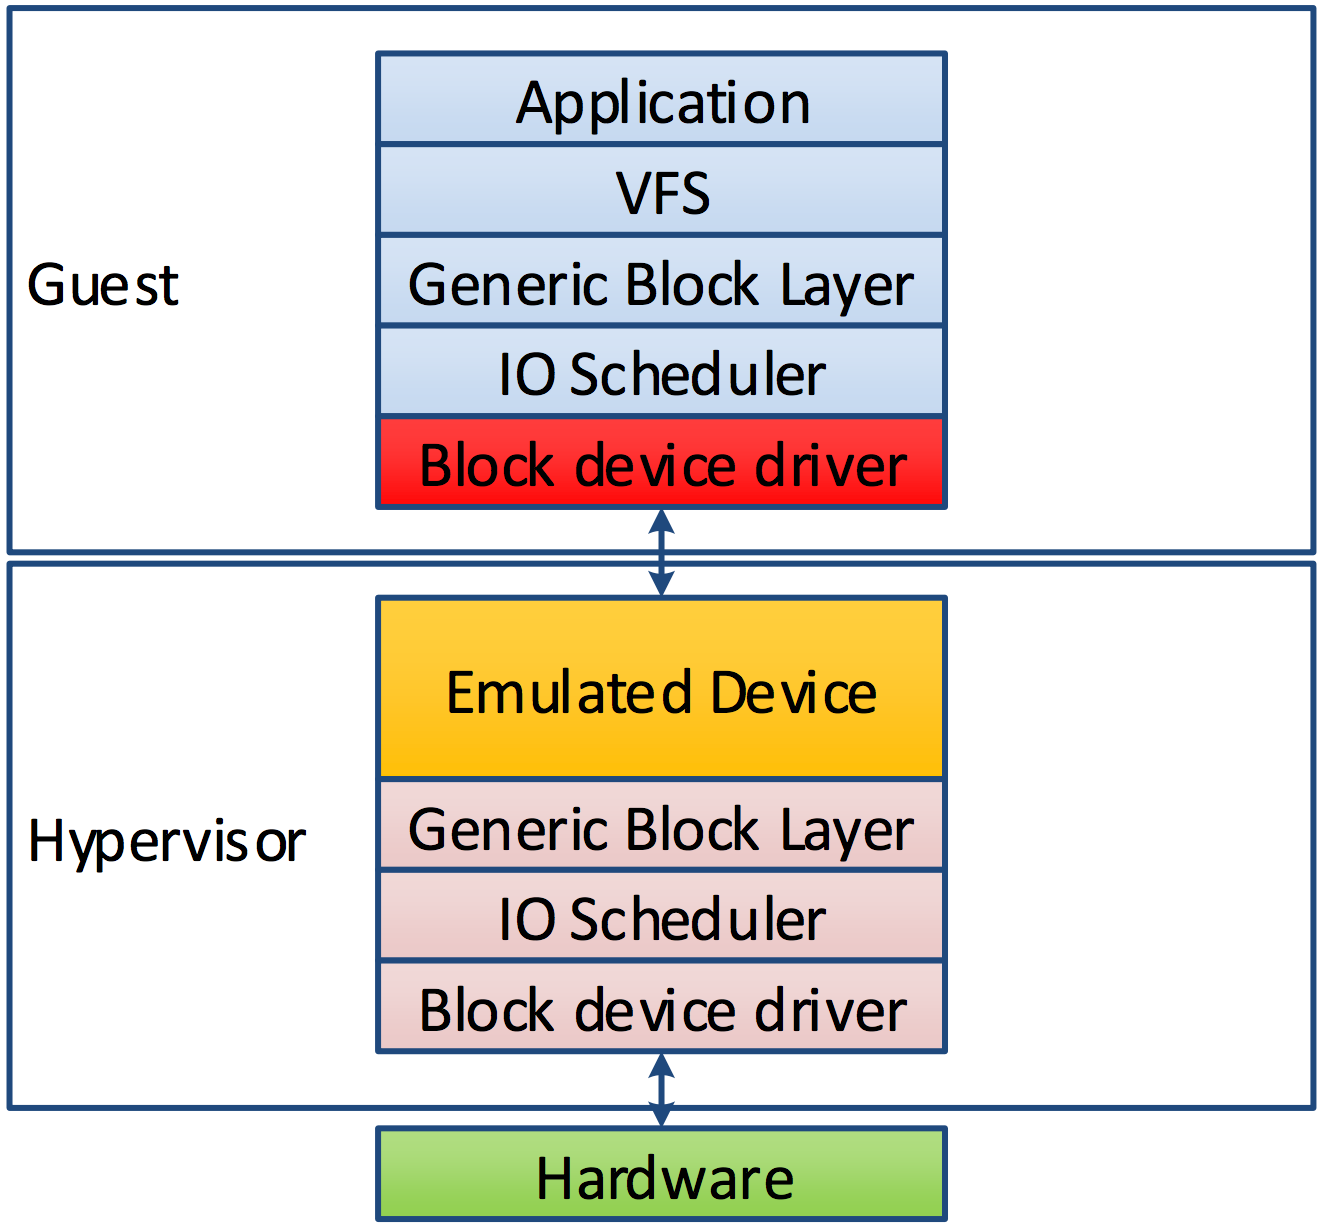
\includegraphics[width=0.3\textwidth]{figs/emulation.png}
      \label{fig:storage:emulation}
    }
    \hfill
    \subfloat[virtio]{
      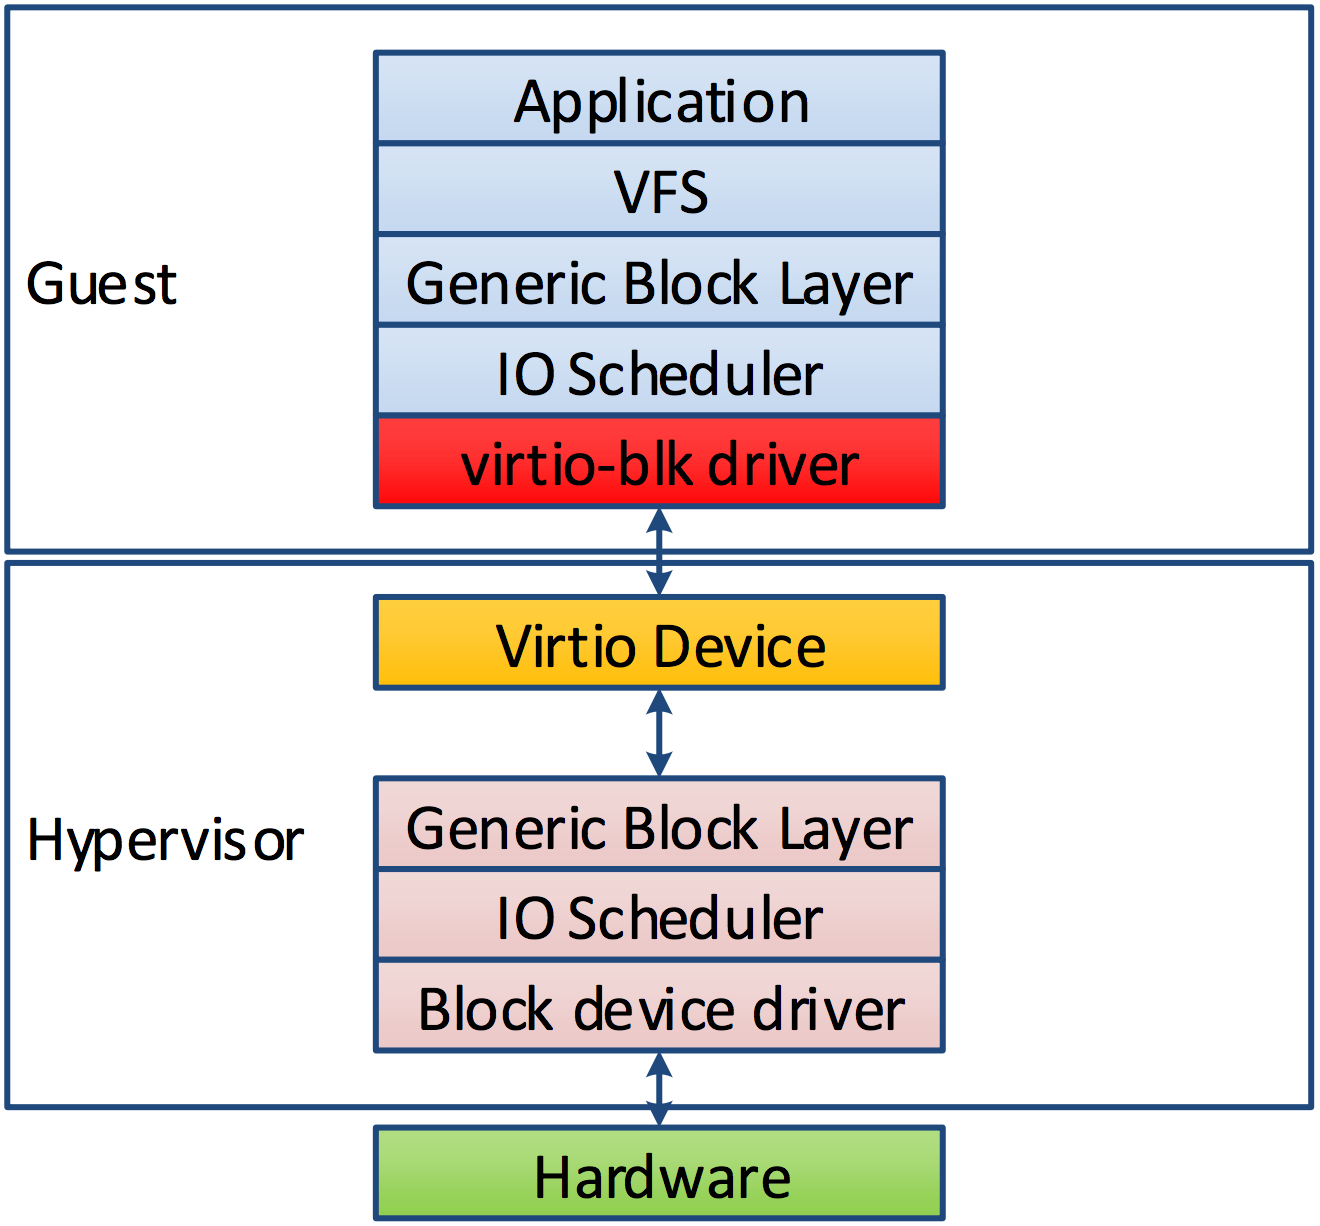
\includegraphics[width=0.3\textwidth]{figs/virtio.png}
      \label{fig:storage:virtio}
    }
    \hfill
    \subfloat[Direct-IO]{
      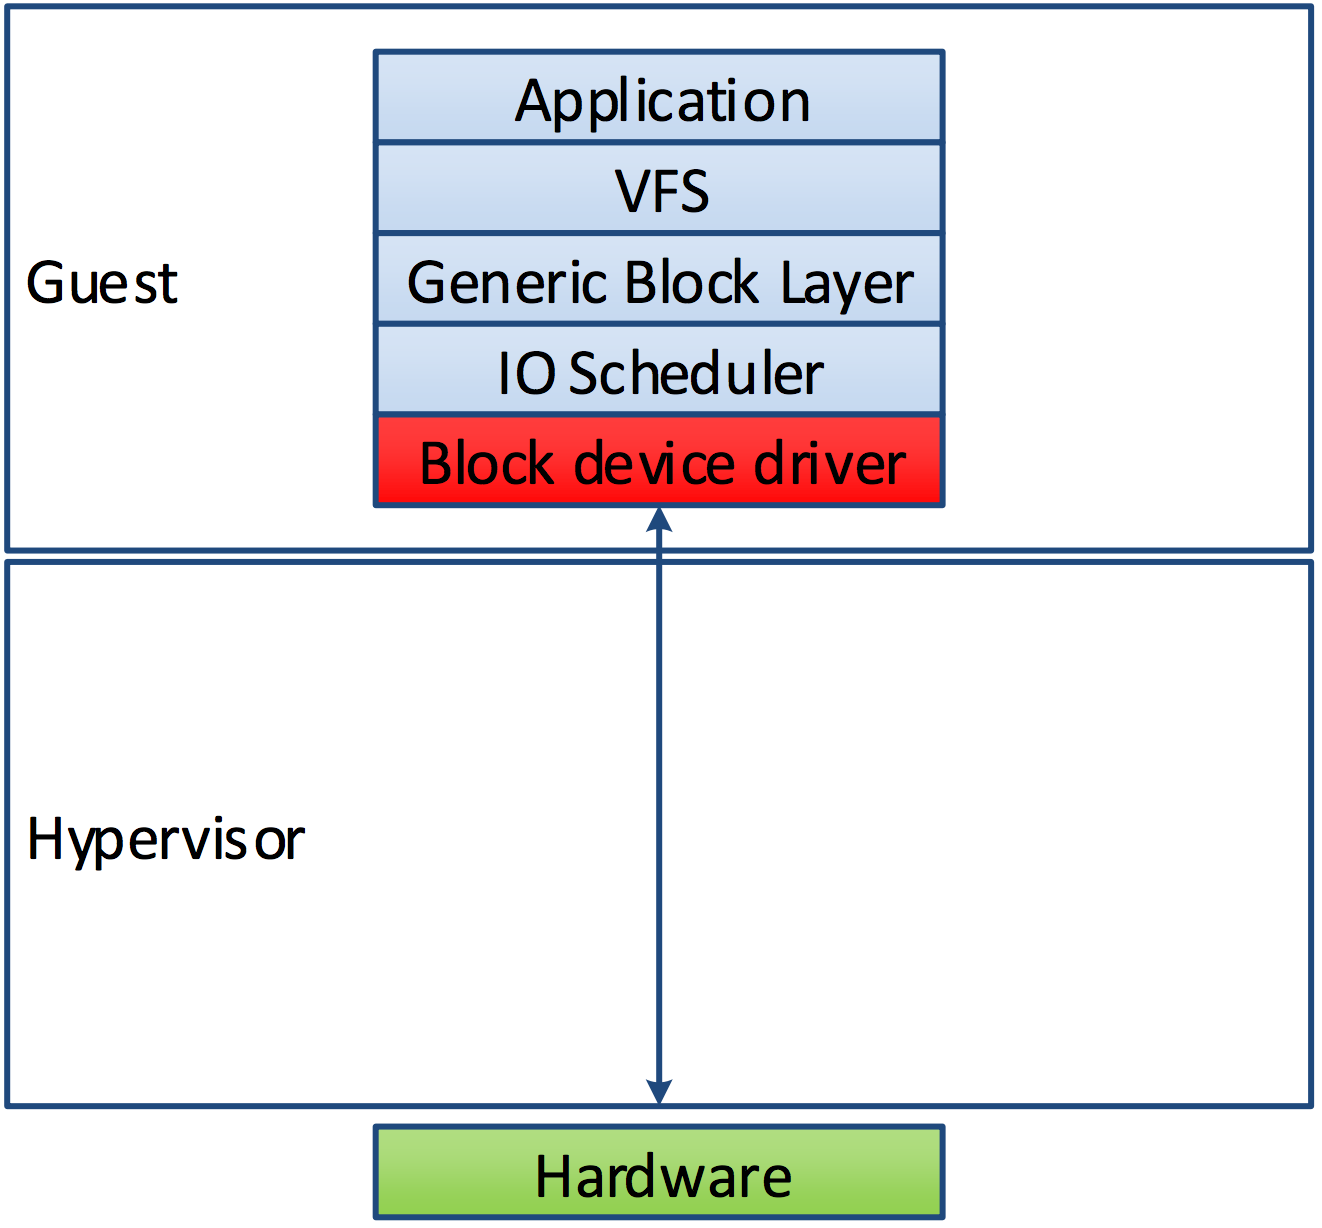
\includegraphics[width=0.3\textwidth]{figs/direct.png}
      \label{fig:storage:direct}
    }
    \caption{IO Virtualization techniques.
      \label{fig:storage}}
    
\end{figure*}




%%%%%%%%%%%%%%%%%%%%%%%%%%%%%%%%%%%%%%%%%%%%%%%%%%
\section{Virtualization Background}
%%%%%%%%%%%%%%%%%%%%%%%%%%%%%%%%%%%%%%%%%%%%%%%%%%
Virtualization is the act of logically dividing the system resources between different entities
running on it. Virtualization hides the physical characteristics of a computing platform from the users,
presenting instead another abstract computing platform. The software that controls the virtualization of the
system is called \emph{hypervisor} or \emph{virtual machine monitor} (VMM).

Virtualization is performed on a given hardware platform by host software (hypervisor), which creates a
simulated computer environment, a virtual machine (VM), for its guest software.
The guest software is not limited to user applications; many hosts allow the execution of complete operating
systems. The guest software executes as if it were running directly on the physical hardware, with several
notable caveats. Access to physical system resources (such as the network access, display, keyboard, and disk
storage) is generally managed at a more restrictive level than the host processor and system-memory. Guests are
often restricted from accessing specific peripheral devices, or may be limited to a subset of the device's
native capabilities, depending on the hardware access policy implemented by the virtualization host.
Virtualization often exacts performance penalties, both in resources required to run the hypervisor,
and as well as in reduced performance on the virtual machine compared to running native on the physical machine.

%%%%%%%%%%%%%%%%%%%%%%%%%%%%%%%%%%%%%%%%%%%%%%%%%%
\subsection*{Virtualization Aspects}
%%%%%%%%%%%%%%%%%%%%%%%%%%%%%%%%%%%%%%%%%%%%%%%%%%
There are three main resources that the hypervisor needs to virtualize: the CPU, Memory and I/O devices.

\paragraph {CPU}
A common implementation of CPU virtualization is \emph{Trap-and-Emulate}. When using this technique,
the guest code (OS or user application) may run directly on the CPU and only when an unprivileged command is
executed, the CPU will issue a trap to the hypervisor that  will emulate the guest command. To configure the instructions that cause a VM to trap, modern CPUs expose a special interface (Intel's VT-x and AMD AMD-V) for the hypervisor to program.


\paragraph {Memory}
Just like any other process running on the system, a guest OS has no control over the hosts physical memory.
The hypervisor will have to provide each of the guest OSs with the illusion of a more or less contiguous block of physical memory starting at address 0, because that's what all OSs expect.
%
The simplest way to do that is to introduce one more level of virtualization, one more  level of mapping between what the guest OS considers a physical address (it's called \emph{guest physical address}) and the actual physical address (which is called \emph{host physical address}).
The hypervisor isolates the running VM with page tables that translate \emph{guest physical address} to \emph{host physical address}. When a guest application is running, each memory access (to \emph{guest virtual address}) must pass two translation layers, the first translates to \emph{guest physical address}, and the second translates to \emph{host physical address}.

Modern processors use \emph{Extended Page Tables} (EPT) technology. This technology enables the \emph{MMU} to do this double translation: First it translates the \emph{guest virtaul address} to \emph{guest physical address} using the page tables set by the guest OS. Then it translates the \emph{guest physical address} to \emph{host physical address} using the page tables set by the hypervisor.

Another technique used on systems without EPT support is called \emph{shadow page tables}. The idea is to create a second copy of VM's page tables called shadow page tables that map \emph{guest virtual addresses} directly to host physical addresses (actual DRAM), and let the processor use them for address translation (so the CR3 register points to those, rather than to guest, or primary page tables).

\paragraph {I/O devices}
Its the hypervisor's responsibility to share an I/O device between virtual machines. When sharing a device, isolation must be enforced so that one VM cannot access other VMs' resources on the same I/O device.
Figure~\ref{fig:storage} illustrates the three most common methods by which hypervisors virtualize storage devices (We discuss storage devices, but the same technologies work for any I/O device ):

\begin{enumerate}
\item
  \emph{Full device emulation}~\cite{sugerman2001virtualizing} (Figure~\ref{fig:storage:emulation})\quad
  In this method, the host emulates a well known hardware device.
  The hypervisor attaches the emulated device to the VM's physical address space (\emph{guest physical address}), and the gust OS will discover the device while scanning the system for physical devices. When the device is discovered
  the OS will load the appropriate driver. Whenever the guest will access the address space representing the device (a PCIe function for example), a trap will be issued by the processor, and the hypervisor will emulate the
  behavior of the device for that access.

  When the device is a block device, the emulated device is represented as a file on the host filesystem. Whenever the guest tries to access a \emph{logical block address} (LBA) on the device, the host converts the LBA to an offset
  in the file, and depending on the command, reads/writes data from/to that offset.

  The advantage of this method is that the guest doesn't require any changes and can run unmodified device drivers.
  The disadvantage is the high latency of each request, that has to pass through all the block I/O software layers in the guest, and then again in the host. 
  The overheads of device emulation is discussed later.

  
\item
  \emph{Paravirtualization}~\cite{barham2003xen,russell2008virtio} (Figure~\ref{fig:storage:virtio})\quad
  This method eliminates the need for the hypervisor to emulate a complete physical device and enables the guest VM to directly request a virtual LBA from the
  hypervisor, thereby improving performance. The hypervisor still emulates a device, but the guest knows the device is emulated and not real and can optimize the interface between it and the hypervisor. 
  This is the most common storage virtualization method used in modern hypervisors.

\item
  \emph{Direct device assignment}~\cite{raj2007high} (Figure~\ref{fig:storage:direct})\quad
  This method allows the guest VM to directly interact with the physical device without hypervisor mediation. 
  Consequently, it delivers the best storage performance to the VM. However, since legacy storage devices do not enforce isolation among clients, it does not allow multiple VMs to share a physical device. The new PCIe protocol's SR-IOV feature
  allows multiple clients to access the same physical device while enforcing isolation at the hardware level. We discuss SR-IOV in section~\ref{sec:sriov}
  

\end{enumerate}


%%%%%%%%%%%%%%%%%%%%%%%%%%%%%%%%%%%%%%%%%%%%%%%%%%
\section{The I/O Stack}
%%%%%%%%%%%%%%%%%%%%%%%%%%%%%%%%%%%%%%%%%%%%%%%%%%
The I/O stack is the set of abstractions an I/O request passes starting at the application
issuing the read/write request, and ending at the data written/read to the physical storage
device.

%%%%%%%%%%%%%%%%%%%%%%%%%%%%%%%%%%%%%%%%%%%%%%%%%%
\subsection*{I/O Stack Components}
%%%%%%%%%%%%%%%%%%%%%%%%%%%%%%%%%%%%%%%%%%%%%%%%%%
%%%%%%%%%%%%%%%%%%%%%%%%%%%%%%%%%%%%%%%%%%%%%%%%%%
\paragraph{Filesystem}
%%%%%%%%%%%%%%%%%%%%%%%%%%%%%%%%%%%%%%%%%%%%%%%%%%
A filesystem is the methods and data structures that an operating system uses to keep track of
files on a disk or partition; that is, the way the files are organized on the disk.
Every filesystem implements a mapping mechanism in which file offsets are mapped to physical
 storage blocks.
Traditionally, UNIX-derived filesystems used per-file direct and indirect  block mapping tables
to map offsets in a file to their corresponding data block. But tracking individual blocks
incurs large spatial and latency overheads when dealing with large files. 
Modern UNIX filesystems (e.g., ext4~\cite{mathur07ext4},btrfs~\cite{rodeh13btrfs},
 xfs~\cite{sweeney96xfs}) therefore group contiguous physical blocks
 into \emph{extents} and construct extent trees, which consist of variants of
 B-trees~\cite{comer79btree}, to spatially map offsets in the device to extents.
Each file is associated with an extent tree (pointed to by the file's \emph{inode}) that maps
 file offsets to physical blocks.

%%%%%%%%%%%%%%%%%%%%%%%%%%%%%%%%%%%%%%%%%%%%%%%%%%
\paragraph{Block Layer}
%%%%%%%%%%%%%%%%%%%%%%%%%%%%%%%%%%%%%%%%%%%%%%%%%%
The block layer is a kernel component that handles the requests for all block devices in the system.
A request can reach this layer either from the filesystem layer, or directly from an application reading/writing straight to the raw device.


%%%%%%%%%%%%%%%%%%%%%%%%%%%%%%%%%%%%%%%%%%%%%%%%%%
\paragraph{Device Driver}
\label{iovirt:driver}
%%%%%%%%%%%%%%%%%%%%%%%%%%%%%%%%%%%%%%%%%%%%%%%%%%
The role of device drivers is to communicate with I/O devices attached to the system.
Block device drivers get block read/write requests from the block layer in the form of a \emph{bio struct}. The bio object contains everything that a block driver needs to carry out the request to
the block device, including the LBA of the request, the size
and the virtual address from where the data is copied from/to.

%%%%%%%%%%%%%%%%%%%%%%%%%%%%%%%%%%%%%%%%%%%%%%%%%%
\paragraph{Block Device}
%%%%%%%%%%%%%%%%%%%%%%%%%%%%%%%%%%%%%%%%%%%%%%%%%%
A block device is a computer data storage device that supports reading and writing data in
fixed-size blocks. These blocks are generally 512 bytes or a multiple thereof in size. The term is often used in contrast with a ``word-addressed device'' which supports reading and
writing data a word at a time, where a "word" is a much smaller block, usually 1 to 8 bytes in size.

%%%%%%%%%%%%%%%%%%%%%%%%%%%%%%%%%%%%%%%%%%%%%%%%%%
\section{Single Root I/O Virtualization}
\label{sec:sriov}
%%%%%%%%%%%%%%%%%%%%%%%%%%%%%%%%%%%%%%%%%%%%%%%%%%
The single root I/O virtualization (SR-IOV) interface is an extension to the PCI Express (PCIe) specification.
SR-IOV allows a device to separate access to its resources among various PCIe hardware functions. These functions consist of the following types:

\begin{itemize}
\item \emph{Physical Function (PF)} \quad
  The PF is a full-featured PCIe function. The PF includes the SR-IOV capability in the PCIe Configuration space.
  The capability is used to configure and manage the SR-IOV functionality of the device, such as enabling
  virtualization and exposing VFs.
\item \emph{Virtual Function (VF)} \quad
  A VF is a lightweight PCIe function that supports the SR-IOV interface. The VF represents a virtualized instance of the physical device.
  Each VF has its own PCI Configuration space. Each VF also shares one or more physical
  resources on the physical device with the PF and other VFs.
\end{itemize}

SR-IOV extends the direct device assignment method discussed earlier to allow multiple virtual machines to directly access the same physical device.
This is done by creating multiple VFs' and attaching each of them to a different VM. Isolation of the resources is done by the device and the hypervisor doesn't
intercept every access done to the device.

\subsubsection{NVM Express}
\label{subsec:nvme}
NVM Express (NVMe) is a logical device interface specification for accessing non-volatile storage media attached via PCI Express (PCIe) bus.
The NVMe specification defines how an SSD device divides its resources among several VFs'. The hypervisor divides the storage blocks into \emph{namespaces}
and defines a mapping between a VF to a \emph{namespace}. When a VM accesses a VF, the requests are translated to the correct \emph{namespace}.





















